\documentclass{beamer}
\usetheme{Madrid}

\usepackage{graphicx}
\usepackage{tabularx}
\usepackage{subfig}
\usepackage{natbib}
\usepackage{tikz}

\title[CDT]{Constrained Delaunay Tetrahedralization(CDT) for applications in Nuclear reactor component modelling}
\author{Pranav Kant Gaur}
\institute[BARC, India]{Computer Division, \newline Bhabha Atomic Research Centre, Mumbai, India}
\titlegraphic{
\includegraphics[width=2cm, height=2cm]{figures/barc_logo.jpg}}
\date{}

\begin{document}
%%%%%%%%%%%%%%%%%%%%%%%%%%%%%%%%%%%%%%%%%%%%%%%%%%%%%%%%%%%%%%%%%%%%%%%%%%%%%%%%%%%%%%%%%%%%%%%%%%%%%%%
	\begin{frame}
		\titlepage
	\end{frame}	
%%%%%%%%%%%%%%%%%%%%%%%%%%%%%%%%%%%%%%%%%%%%%%%%%%%%%%%%%%%%%%%%%%%%%%%%%%%%%%%%%%%%%%%%%%%%%%%%%%%%%%%
	\begin{frame}
		\frametitle{Motivation}
			\begin{itemize}
				\item CFD analysis for Nuclear reactor component modelling:
					\begin{itemize}
						\item Designing reactor core:
							\begin{figure}
								\begin{tabularx}{\linewidth}{@{}cXX@{}}
									\begin{tabular}{c c c}
										\hspace{-2cm}\subfloat[]{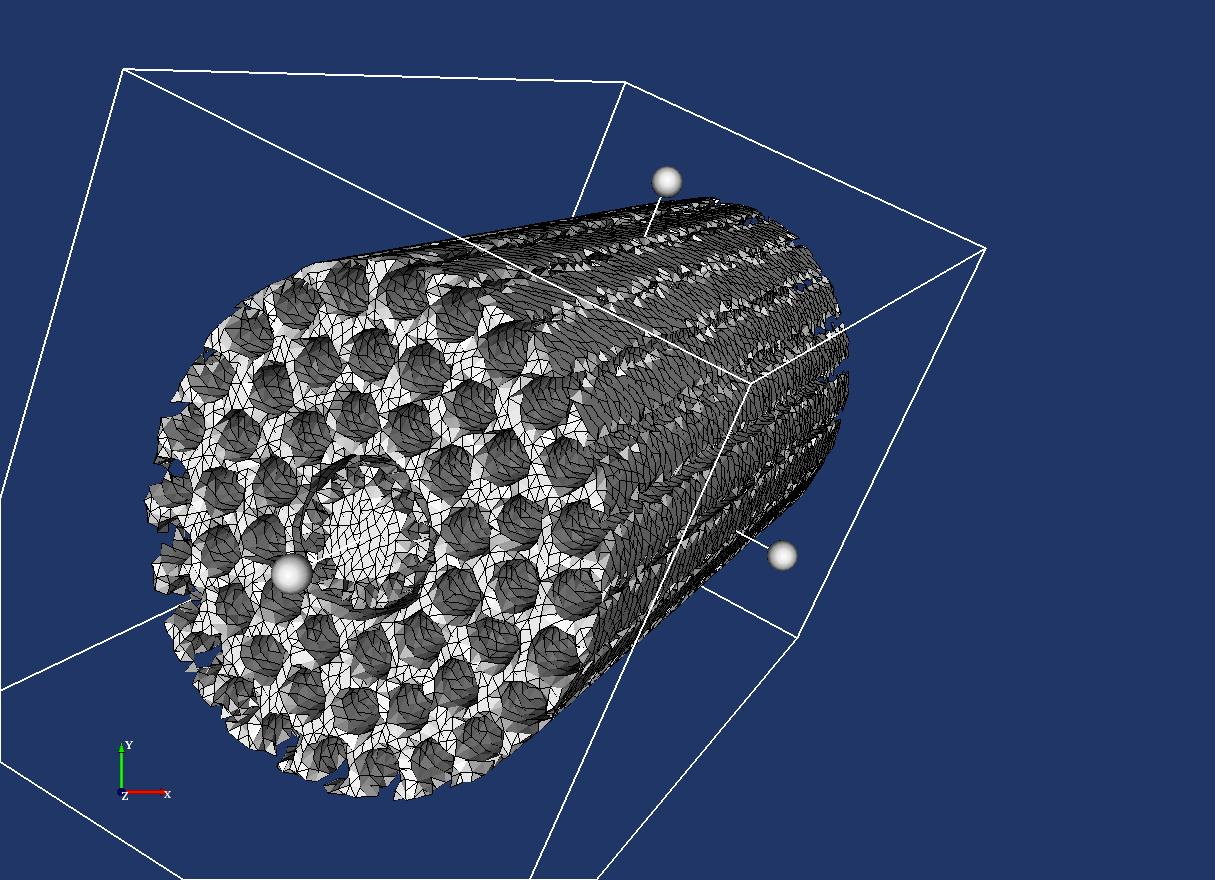
\includegraphics[width=4cm, height=3cm]{figures/fuelView1.jpg}} &
										\subfloat[]{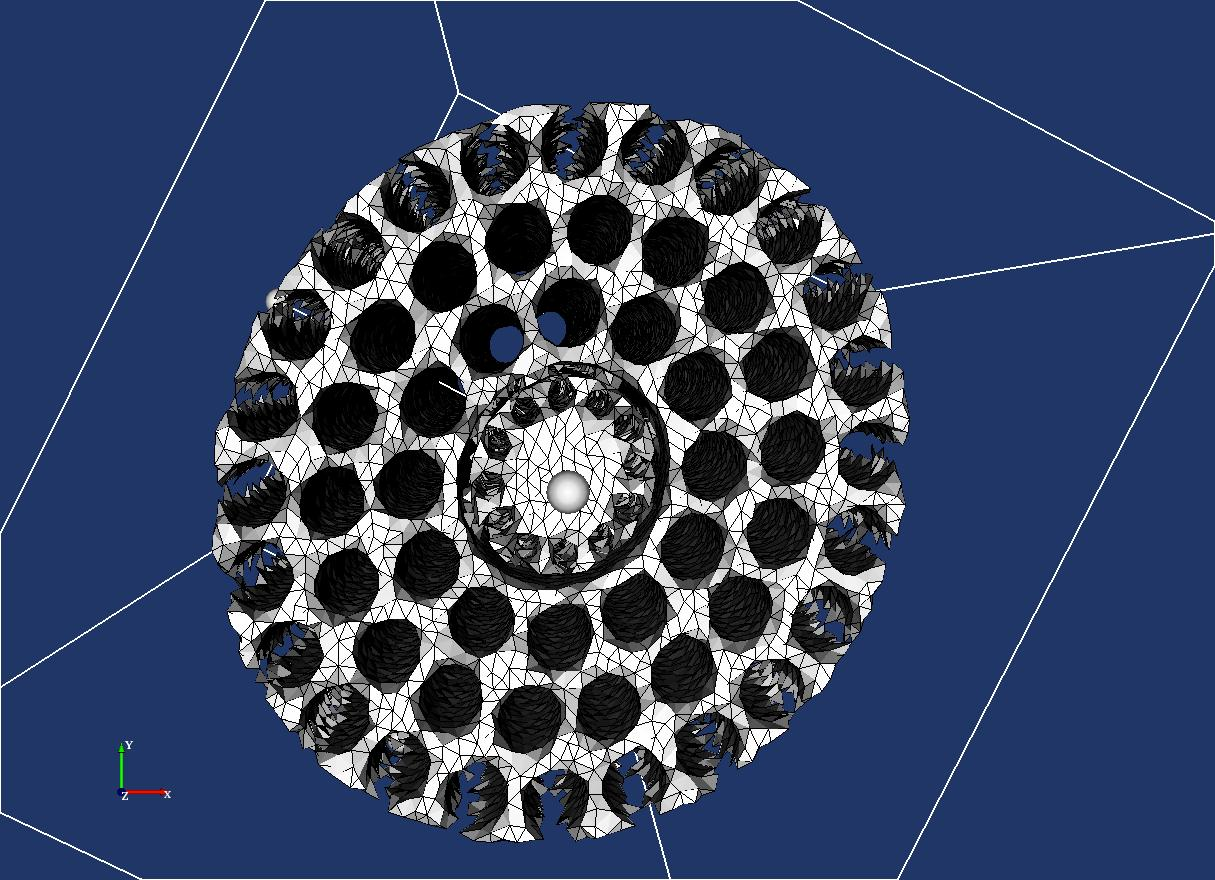
\includegraphics[width=4cm, height=3cm]{figures/fuelView2.jpg}} &
										\subfloat[]{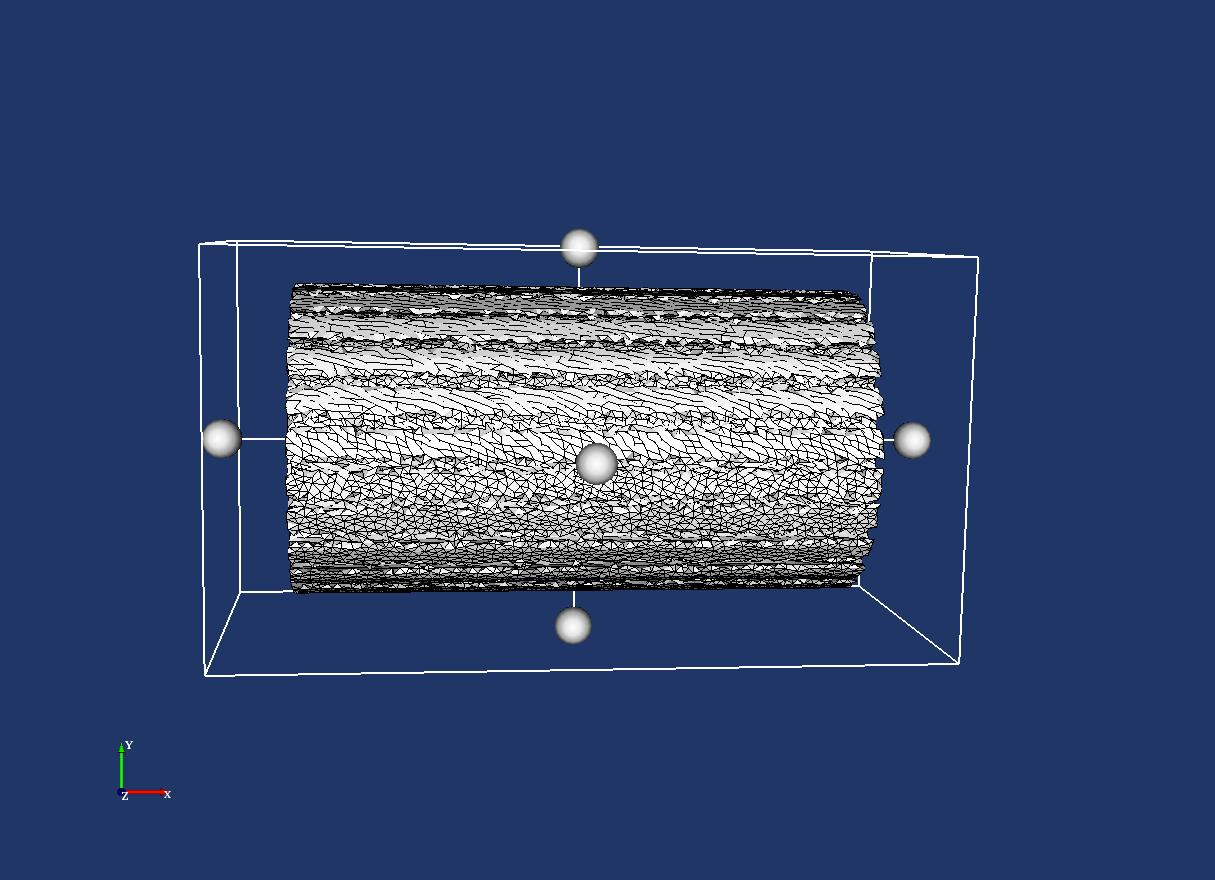
\includegraphics[width=4cm, height=3cm]{figures/fuelView3.jpg}} \\
									\end{tabular}
								\end{tabularx}	
								\caption{Fuel bundle}
							\end{figure}	
					\end{itemize}		
			\end{itemize}
	\end{frame}
%%%%%%%%%%%%%%%%%%%%%%%%%%%%%%%%%%%%%%%%%%%%%%%%%%%%%%%%%%%%%%%%%%%%%%%%%%%%%%%%%%%%%%%%%%%%%%%%%%%%%%%
	\begin{frame}
		\frametitle{Motivation(contd.)}
			\begin{itemize}
				\item Anupravaha
					\begin{itemize}
						\item General purpose CFD solver over hybrid unstructured grid.
						\item Collaboration project between BARC and other academic institutions.
						\item Integrated mesh generation and CFD solver:
							\begin{itemize}
								\item Currently, no open source software  with iterative feedback based hybrid mesh generation capability.
								\item Need to have tighter control over configurability of mesh generation and solver tools.	
							\end{itemize}	
					\end{itemize}		
			\end{itemize}		
	\end{frame}	
%%%%%%%%%%%%%%%%%%%%%%%%%%%%%%%%%%%%%%%%%%%%%%%%%%%%%%%%%%%%%%%%%%%%%%%%%%%%%%%%%%%%%%%%%%%%%%%%%%%%%%%
	\begin{frame}	
		\frametitle{Motivation(contd.)}	
			\begin{itemize}
				\item Resulting mesh should have elements suitable for finite element calculations:
					\begin{itemize}
						\item Constrained Delaunay Tetrahedralization is optimal domain discretization approach for Finite element applications \cite{schewFiniteElements}.
							\begin{itemize}
								\item Preserves input domain in output mesh.
								\item Shares characterstics with Delaunay triangulation \cite{schewCDTExistence}	
								\item Maximizes minimum dihedral angle(\textit{Delaunay property}) \cite{schewFiniteElements}.
							\end{itemize}
					\end{itemize}		
			\end{itemize}		
	\end{frame}
%%%%%%%%%%%%%%%%%%%%%%%%%%%%%%%%%%%%%%%%%%%%%%%%%%%%%%%%%%%%%%%%%%%%%%%%%%%%%%%%%%%%%%%%%%%%%%%%%%%%%%%%
	\begin{frame}
		\frametitle{Constrained Delaunay Tetrahedralization}
			\begin{itemize}
				\item Simplical complex: A topological space formed by gluing together points, line segments, triangles and their $n$-dimensional counterparts.	
				\item A simplical complex is \textit{constrained Delaunay} if there exist a circumsphere which encloses no other \textit{visible} point inside it.
					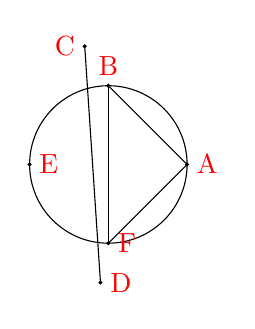
\begin{tikzpicture}
						\draw (1, 0) -- (0, 1); %label these points
						\draw (0, 1) -- (0, -1);
						\draw (1, 0) -- (0, -1);
						\draw (0, 0) circle (1cm);
						\filldraw (1, 0) circle[radius=0.5pt];
						\filldraw (0, 1) circle[radius=0.5pt];
						\filldraw (0, -1) circle[radius=0.5pt];
						\filldraw (-1, 0) circle[radius=0.5pt];
						\draw (-0.3, 1.5) -- (-0.1, -1.5);
						\filldraw (-0.3, 1.5) circle[radius=0.5pt];
						\filldraw (-0.1, -1.5) circle[radius=0.5pt];
						\node [red, right] at (1, 0) {A};
						\node [red, above] at (0, 1) {B};					
						\node [red, left] at (-0.3, 1.5) {C};					
						\node [red, right] at (-0.1, -1.5) {D};
						\node [red, right] at (-1, 0) {E};					
						\node [red, right] at (0, -1) {F};					
					\end{tikzpicture}	
				\item Constrained Delaunay Tetrahedralization is a simplical complex of constrained Delunay cells.
			\end{itemize}
	\end{frame}	
%%%%%%%%%%%%%%%%%%%%%%%%%%%%%%%%%%%%%%%%%%%%%%%%%%%%%%%%%%%%%%%%%%%%%%%%%%%%%%%%%%%%%%%%%%%%%%%%%%%%%%%%%
	\begin{frame}
		\frametitle{Theoretical underpinnings}
			\begin{itemize}
				\item	Schewchuck's CDT existence theorem \cite{schewCDTExistence}:
					\begin{itemize}
						\item  A PLC $X$ has a $d$-dimensional CDT if each $k$-dimensional constraining facet in $X$ with $k \leq d -2$ is a union of strongly Delaunay $k$-simplices.								
							\begin{figure}
								\begin{tabularx}{\linewidth}{@{}cXX@{}}
									\begin{tabular}{c c c}
										\subfloat[$D$ is inside: Not strongly Delaunay]{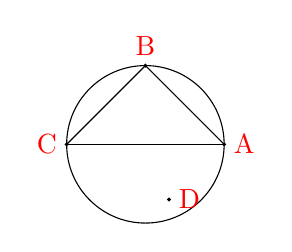
\begin{tikzpicture}
											\draw (1, 0) -- (0, 1); %label these points
											\draw (0, 1) -- (-1, 0);
											\draw (1, 0) -- (-1, 0);
											\draw (0, 0) circle (1cm);
											\filldraw (1, 0) circle[radius=0.5pt];
											\filldraw (0, 1) circle[radius=0.5pt];
											\filldraw (-1, 0) circle[radius=0.5pt];
											\filldraw (0.3, -0.7) circle[radius=0.5pt];
											\node [red, right] at (1, 0) {A};
											\node [red, above] at (0, 1) {B};		
											\node [red, left] at (-1, 0) {C};
											\node [red, right] at (0.3, -0.7) {D};
											\end{tikzpicture}} &
										\subfloat[$D$ is on boundary: Not strongly Delaunay]{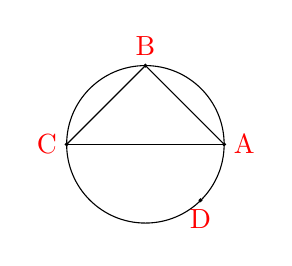
\begin{tikzpicture}
											\draw (1, 0) -- (0, 1); %label these points
											\draw (0, 1) -- (-1, 0);
											\draw (1, 0) -- (-1, 0);
											\draw (0, 0) circle (1cm);
											\filldraw (1, 0) circle[radius=0.5pt];
											\filldraw (0, 1) circle[radius=0.5pt];
											\filldraw (-1, 0) circle[radius=0.5pt];
											\filldraw (0.70, -0.71) circle[radius=0.5pt];
											\node [red, right] at (1, 0) {A};
											\node [red, above] at (0, 1) {B};		
											\node [red, left] at (-1, 0) {C};
											\node [red, below] at (0.70, -0.71) {D};
											\end{tikzpicture}} &
										\subfloat[Strongly Delaunay]{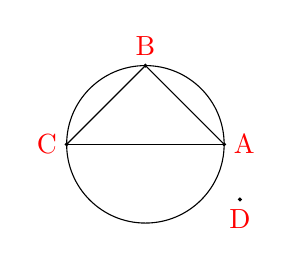
\begin{tikzpicture}
											\draw (1, 0) -- (0, 1); %label these points
											\draw (0, 1) -- (-1, 0);
											\draw (1, 0) -- (-1, 0);
											\draw (0, 0) circle (1cm);
											\filldraw (1, 0) circle[radius=0.5pt];
											\filldraw (0, 1) circle[radius=0.5pt];
											\filldraw (-1, 0) circle[radius=0.5pt];
											\filldraw (1.2, -0.7) circle[radius=0.5pt];
											\node [red, right] at (1, 0) {A};
											\node [red, above] at (0, 1) {B};		
											\node [red, left] at (-1, 0) {C};
											\node [red, below] at (1.2, -0.7) {D};
											\end{tikzpicture}} \\ 	
									\end{tabular}	
								\end{tabularx}
							\end{figure}	
					\end{itemize}	
			\end{itemize}
	\end{frame}				
%%%%%%%%%%%%%%%%%%%%%%%%%%%%%%%%%%%%%%%%%%%%%%%%%%%%%%%%%%%%%%%%%%%%%%%%%%%%%%%%%%%%%%%%%%%%%%%%%%%%%%%%%%
	\begin{frame}	
		\frametitle{Theoretical underpinnings(contd.)}
			\begin{itemize}
				\item	Hang Si's Theorem \cite{hangSiMeshingPLCByCDT}
					\begin{itemize}
						\item If X has no local degeneracy and DT of X contains all segments of X, then CDT of X exists.						
							\begin{figure}
								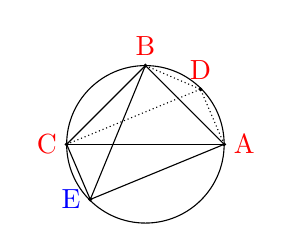
\begin{tikzpicture}
									\draw (1, 0) -- (0, 1); %label these points
									\draw (0, 1) -- (-1, 0);
									\draw (1, 0) -- (-1, 0);
									\draw [densely dotted] (1, 0) -- (0.7, 0.7); % dotted
									\draw [densely dotted] (0, 1) -- (0.7, 0.7);
									\draw [densely dotted] (-1, 0) -- (0.7, 0.7);
									\draw  (1, 0) -- (-0.7, -0.7); % dotted
									\draw  (0, 1) -- (-0.7, -0.7);
									\draw  (-1, 0) -- (-0.7, -0.7);
									\draw (0, 0) circle (1cm);
									\filldraw (1, 0) circle[radius=0.5pt];
									\filldraw (0, 1) circle[radius=0.5pt];
									\filldraw (-1, 0) circle[radius=0.5pt];
									\filldraw (0.7, 0.7) circle[radius=0.5pt];
									\filldraw (-0.7, -0.7) circle[radius=0.5pt];
									\node [red, right] at (1, 0) {A};
									\node [red, above] at (0, 1) {B};		
									\node [red, left] at (-1, 0) {C};
									\node [red, above] at (0.7, 0.7) {D};
									\node [blue, left] at (-0.7, -0.7) {E};
									%\node [blue, right] at () {F};
								\end{tikzpicture}
								\caption{\textbf{Local degeneracy}: $ABCD$ and $ABCE$ are neighbouring Delaunay tetrahedrons}
							\end{figure}	
						\item Does not require constraints to be strongly Delaunay \textit{globally}.
					\end{itemize}		
			\end{itemize}		
	\end{frame}	
%%%%%%%%%%%%%%%%%%%%%%%%%%%%%%%%%%%%%%%%%%%%%%%%%%%%%%%%%%%%%%%%%%%%%%%%%%%%%%%%%%%%%%%%%%%%%%%%%%%%%%%%%
	\begin{frame}
		\frametitle{Hang Si's algorithm} 
			\begin{enumerate}
				\item Transform X into a \textit{topologically equivalent} X' which satisfies preconditions for Si's theorem:	
				\begin{enumerate}
					\item Compute initial Delaunay Tetrahedralization	
					\item Recover constraint segments
						\begin{itemize}
							\item Split constraint segments such that resulting subsegments are \textit{Delaunay}.	
						\end{itemize}	
					\item Remove local degeneracies
						\begin{itemize}
							\item Use symbolic perturbation scheme.
						\end{itemize}		
				\end{enumerate}
				\item Recover constraint facets
					\begin{itemize}
						\item Cavity retetrahedralization.	
					\end{itemize}		
			\end{enumerate}		
	\end{frame}
%%%%%%%%%%%%%%%%%%%%%%%%%%%%%%%%%%%%%%%%%%%%%%%%%%%%%%%%%%%%%%%%%%%%%%%%%%%%%%%%%%%%%%%%%%%%%%%%%%%%%%%%%
	\begin{frame}
		\frametitle{Implementation}
			\textbf{CDTGenerator class}:
				\begin{itemize}
					\item Data members:
						\begin{itemize}
							\item plc : input piecewise linear complex
							\item DT : intermidiate Delaunay triangulation
							\item cdtMesh : output mesh	
						\end{itemize}
					\item Member functions: 
						\begin{itemize}
							\item generate() : \textit{public interface}
								\begin{enumerate}
									\item readInputPLC()
									\item computeDelaunayTetrahedralization()
									\item recoverConstraintSegments()
									\item removeLocalDegeneracies()
									\item recoverConstraintFacets()
									\item removeExteriorTeterahedrons()	
								\end{enumerate}
						\end{itemize}
				\end{itemize}
	\end{frame}	
%%%%%%%%%%%%%%%%%%%%%%%%%%%%%%%%%%%%%%%%%%%%%%%%%%%%%%%%%%%%%%%%%%%%%%%%%%%%%%%%%%%%%%%%%%%%%%%%%%%%%%%%
	\begin{frame}
		\frametitle{Implementation(contd.)}
			\begin{itemize}
				\item Unit tests using Google test:
					\begin{itemize}
						\item Constraint segment recovery and Constraint facet recovery:
							\begin{itemize}
								\item Checks if all constraint segments and constraint facets are recovered.
							\end{itemize}	
					\end{itemize}		
				\item Doxygen inline code documentation
				\item Continous integration testing on Travis CI	
				\item Github repository: https://github.com/pranavkantgaur/CDTGenerator
			\end{itemize}
	\end{frame}	
%%%%%%%%%%%%%%%%%%%%%%%%%%%%%%%%%%%%%%%%%%%%%%%%%%%%%%%%%%%%%%%%%%%%%%%%%%%%%%%%%%%%%%%%%%%%%%%%%%%%%%%%
	\begin{frame}
		\frametitle{Implementation: Using CGAL}
			\begin{itemize}
				\item Geometric object generator package:
					\begin{itemize}
						\item Generating random ray for performing inside-outside test.	
					\end{itemize}
				\item Combinatorial Maps and Linear Cell complex packgage:
					\begin{itemize}
						\item Representating Piecewise linear complex and output mesh.	
					\end{itemize}
				\item 3D Triangulations package:
					\begin{itemize}
						\item Representing intermidiate Delaunay triangulations.	
					\end{itemize}		
				\item 2D and 3D Linear Geometry Kernel:
					\begin{itemize}
						\item Points, Triangles, Rays.	
					\end{itemize}		
			\end{itemize}		
	\end{frame}	
%%%%%%%%%%%%%%%%%%%%%%%%%%%%%%%%%%%%%%%%%%%%%%%%%%%%%%%%%%%%%%%%%%%%%%%%%%%%%%%%%%%%%%%%%%%%%%%%%%%%%%%%
	\begin{frame}
		\frametitle{Results} 	
		\textbf{Plateform}: Core i3, 4GB RAM, 3.2 GHZ CPU running Ubuntu 14.04 X86\_64.	
			\begin{itemize}
				\item Cube model:
					\begin{itemize}
						\item Passes unit tests, executes.
							\begin{figure}
								\begin{tabularx}{\linewidth}{@{}cXX@{}}
									\begin{tabular}{c c}
										\hspace{-1.5cm}\subfloat[Input: Cube surface mesh]{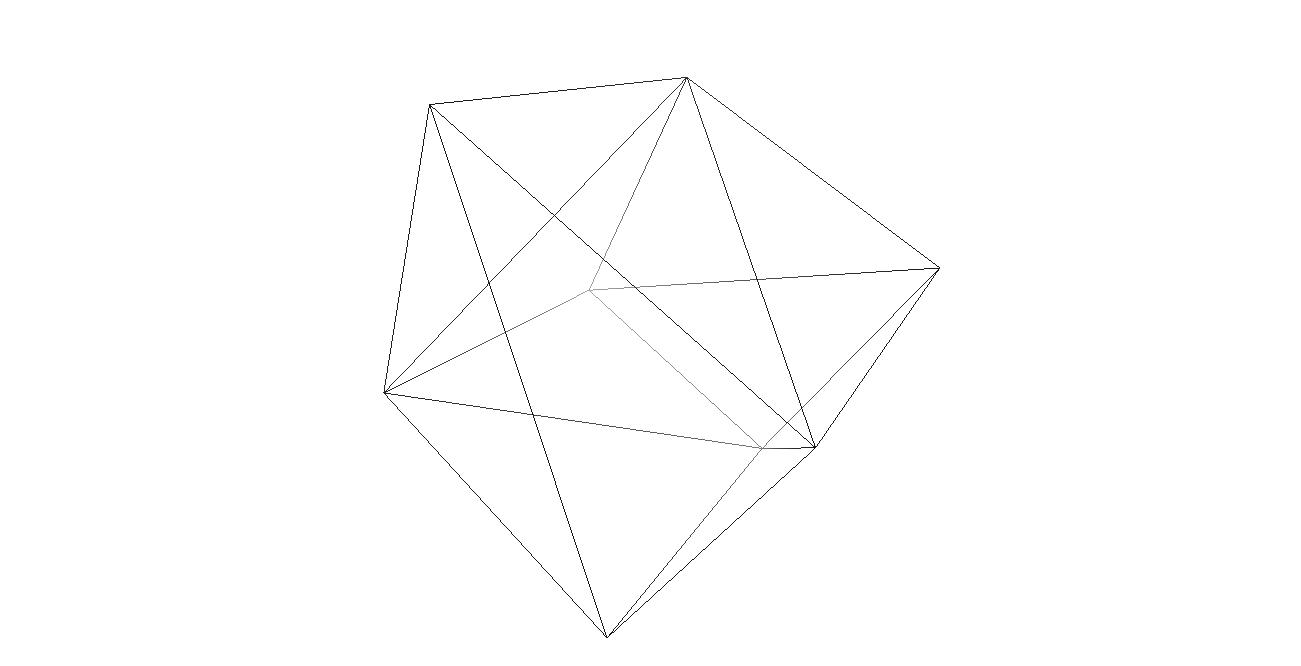
\includegraphics[width=6cm, height=3cm]{figures/cubeInput.jpg}} &
										\subfloat[Output: Cube tetrahedral mesh]{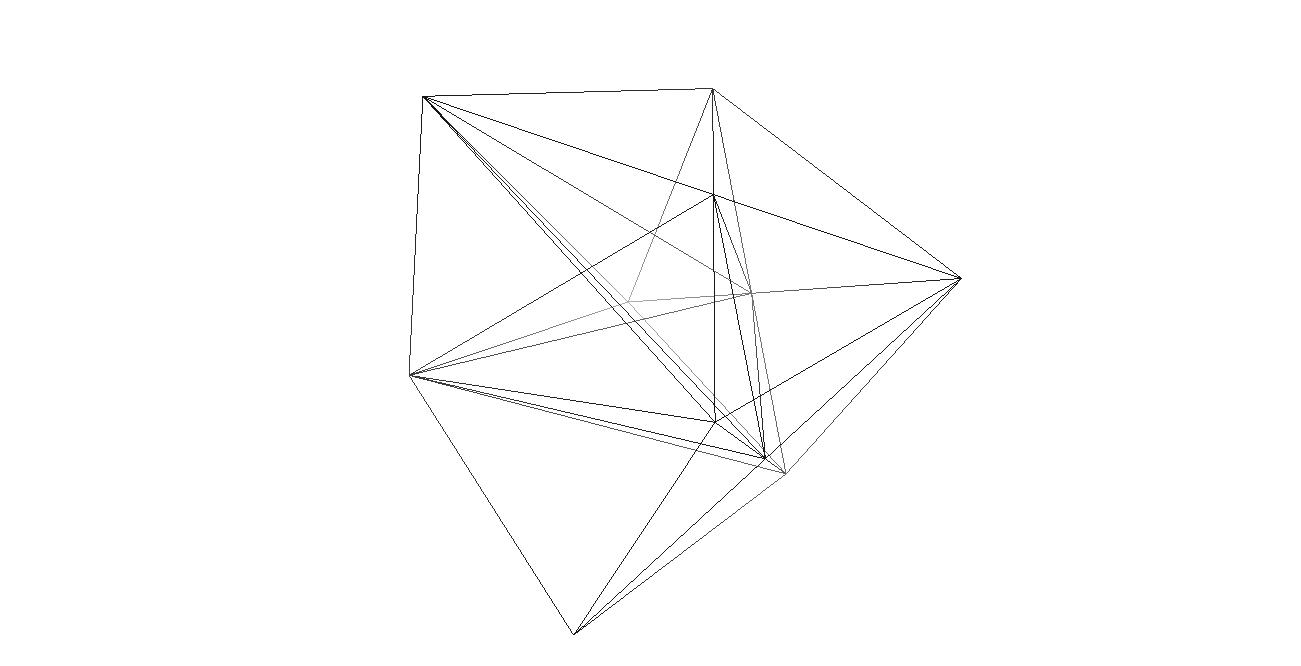
\includegraphics[width=6cm, height=3cm]{figures/cubeOutput.jpg}} \\
									\end{tabular}
								\end{tabularx}	
							\end{figure}	
					\end{itemize}
				\item Sphere model:
					\begin{itemize}
						\item Does not terminate in call to remove exterior tetrahedrons from output mesh.
						\item Takes more than 10 minutes in facet recovery step(\textit{unacceptable}).
					\end{itemize}		
			\end{itemize}		
	\end{frame}	
%%%%%%%%%%%%%%%%%%%%%%%%%%%%%%%%%%%%%%%%%%%%%%%%%%%%%%%%%%%%%%%%%%%%%%%%%%%%%%%%%%%%%%%%%%%%%%%%%%%%%%%%%
	\begin{frame}
		\frametitle{TODOs}
			\begin{itemize}
				\item Devise efficient algorithm for checking if a 3-cell is inside Linear cell complex.
				\item Extend the code for adaptive mesh generation with feedback loop from CFD solver. 
				\item Generalize the solution to support Hybrid meshing. 		
			\end{itemize}
		\end{frame}	
%%%%%%%%%%%%%%%%%%%%%%%%%%%%%%%%%%%%%%%%%%%%%%%%%%%%%%%%%%%%%%%%%%%%%%%%%%%%%%%%%%%%%%%%%%%%%%%%%%%%%%%%%
	\begin{frame}
		\hspace{3cm}\Huge \textbf{Thank you!!}
	\end{frame}	
%%%%%%%%%%%%%%%%%%%%%%%%%%%%%%%%%%%%%%%%%%%%%%%%%%%%%%%%%%%%%%%%%%%%%%%%%%%%%%%%%%%%%%%%%%%%%%%%%%%%%%%%%
\begin{frame}
	\frametitle{References}
		\bibliography{INRIAbib}
		\bibliographystyle{plain}
\end{frame}
%%%%%%%%%%%%%%%%%%%%%%%%%%%%%%%%%%%%%%%%%%%%%%%%%%%%%%%%%%%%%%%%%%%%%%%%%%%%%%%%%%%%%%%%%%%%%%%%%%%%%%%%%%
\end{document}
